\section{Aufteilung der Arbeitspakete}

\begin{figure}[h!]
    \centering
    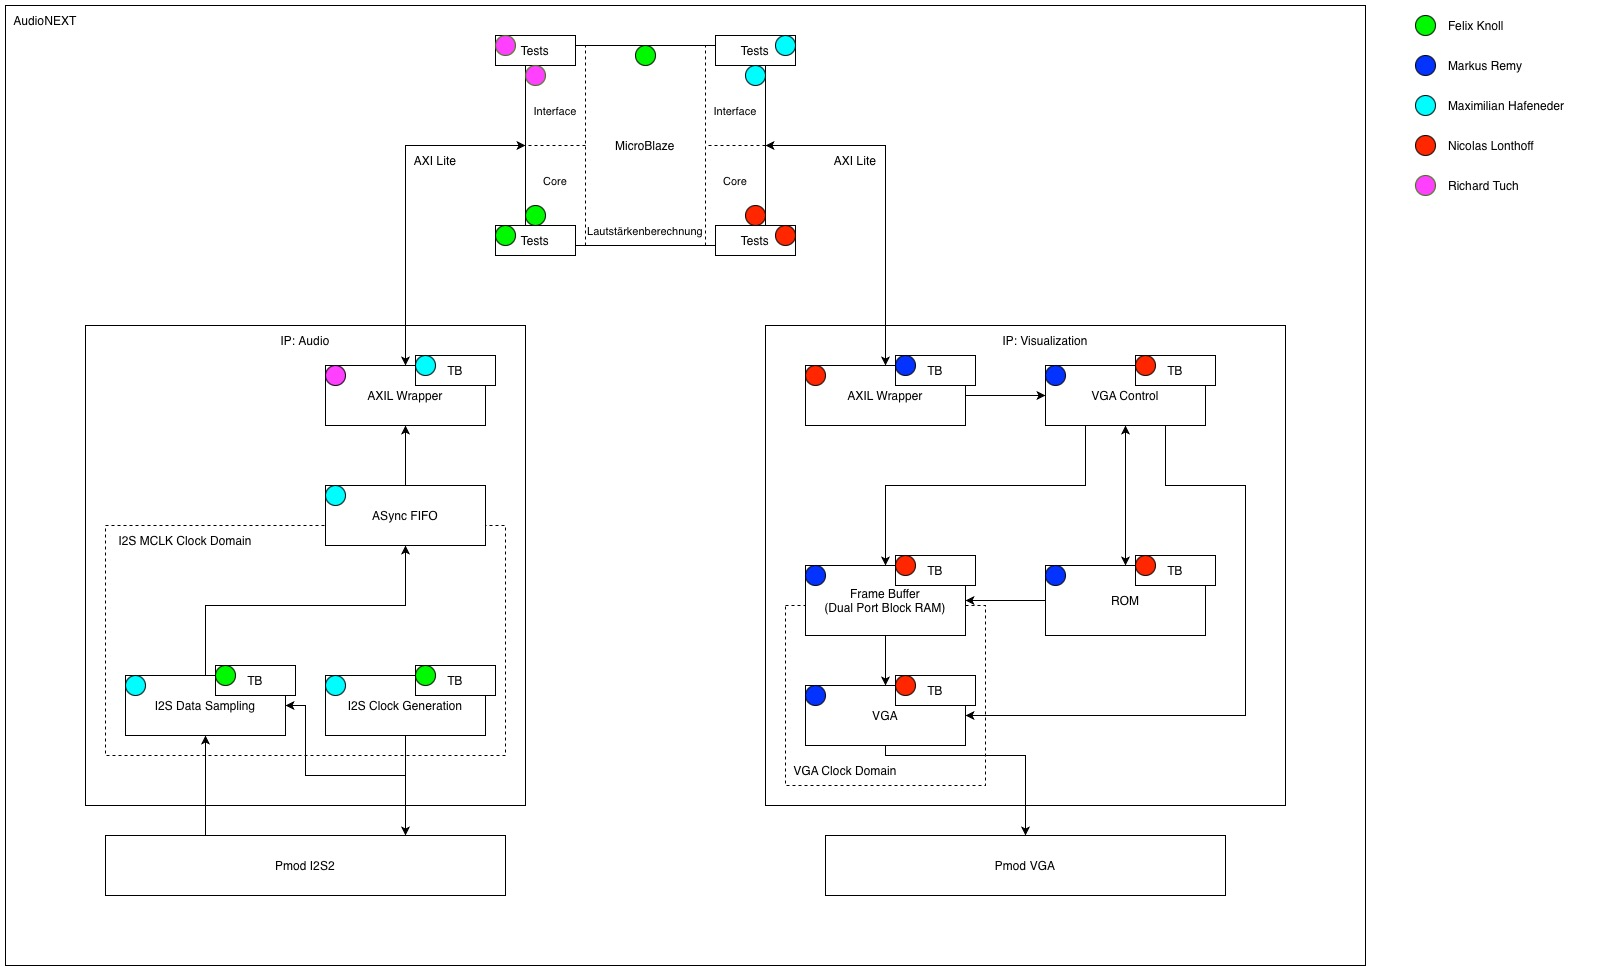
\includegraphics[width=1\textwidth]{files/AudioNEXT_WorkloadSplit}
    \label{fig:workload_split_diagram}
\end{figure}

Bei der Hardware wurde als Ansatz \glqq Blackbox Testing\grqq\ verwendet.
Die Module werden somit nicht vom Entwickler des Moduls, sondern von einer anderen Person getestet.
\newline
Die Softwarepakete werden vom jeweiligen Autor getestet.
\newline
Der Audio-Core wird von Maximilian Hafeneder entwickelt und von Felix Knoll getestet.
Der zugehörige AXI Wrapper wird von Richard Tuch entwickelt und von Maximilian Hafeneder getestet.
\newline
Den Visualization-Core entwickelt Markus Remy.
Getestet wird er von Nicolas Lonthoff.
Der zugehörige AXI Wrapper wird gegengleich von Nicolas und Markus entwickelt.
\newline
Das softwareseitige Interface des Audio IPs entwickelt Richard Tuch inklusive der zugehörigen Tests der Register.
Den darüber liegenden Core für den IP entwickelt Felix Knoll ebenfalls inklusive des zughörigen Funktionstests.
\newline
Das softwareseitige Interface des Visualization IPs entwickelt Maximilian Hafeneder inklusive der zugehörigen Tests der Register.
Den darüber liegenden Core für den IP entwickelt Nicolas Lonthoff ebenfalls inklusive des zughörigen Funktionstests.
\newline
Das Hauptprogramm entwickelt Felix Knoll.
\newline
Die Integration des Gesamtsystems wird von Markus Remy angeleitet und mit dem gesamten Team umgesetzt.